\label{sec:catalog-cart}
\subsubsection{Tải menu và trạng thái giao diện}
MenuPage là Server Component gọi GET /products qua lớp API. ProductGrid hiển thị lưới responsive, ProductCard dẫn tới chi tiết theo id; danh sách rỗng có thông báo riêng, lỗi kết nối có nút tải lại. loading.tsx cung cấp khung chờ khi route tải dữ liệu. ProductImage dùng ảnh sản phẩm và minh họa dự phòng khi URL rỗng/ảnh lỗi, tránh đưa src rỗng vào thẻ img.

\subsubsection{Tùy chọn và giá hiển thị}
GET /products/:id cung cấp giá và danh mục phụ thu size/topping từ backend. ProductDetail giữ size, toppings, qty bằng state cục bộ, dùng calcUnitPrice để phản hồi ngay khi chọn. Ví dụ Cappuccino 45.000đ, size L thêm 10.000đ, một topping thêm 5.000đ thành 60.000đ. Availability theo tổ hợp hỗ trợ khóa lựa chọn thiếu nguyên liệu; đây là thông tin tại thời điểm đọc, không giữ hàng trong giỏ. Giá và lượng kho được backend kiểm lại khi tạo đơn như mục~\ref{sec:inventory-requirements}.

\subsubsection{State giỏ hàng và lưu qua lần tải lại}
Zustand lưu items, còn tổng tiền và badge được suy ra qua selector để không có nhiều bản sao tổng cần đồng bộ. Khóa dòng giỏ kết hợp productId, size và danh sách topping đã sort: cùng lựa chọn gộp số lượng, khác size/topping tách dòng. setQty cập nhật số lượng hoặc xóa khi về 0, giới hạn thao tác thông thường ở 99 ly/dòng.

persist lưu giỏ vào localStorage; useHydrated dùng snapshot server/client để tránh render số lượng lưu ở trình duyệt trước khi dữ liệu đó sẵn sàng. Đây là giỏ phía client theo origin, không phải một Order hoặc dữ liệu kho đã được giữ. Không tin unitPrice trong storage là giá thanh toán cuối.

\subsubsection{Gửi đặt hàng và khôi phục khi mất phản hồi}
CartView kiểm đăng nhập, chuyển tới login có next=/cart khi cần; khi đặt, chỉ gửi productId/size/topping/qty và mã voucher. placingRef chặn gửi chồng trong một component. prepareCheckoutIntent lưu key/nội dung theo tài khoản trong sessionStorage trước khi gửi: cùng nội dung sau mất phản hồi dùng lại key, không âm thầm tạo đơn mới. Backend idempotency vẫn là lớp bảo đảm như phần tạo đơn.

Chỉ sau response xác nhận Order, client xóa giỏ, hoàn tất intent và chuyển tới trang đơn. Nếu lỗi hoặc chưa rõ kết quả, giữ ý định để kiểm tra/retry phù hợp. SessionStorage không chứa token của intent; token đăng nhập được lớp auth quản lý riêng. Việc tính giá frontend hỗ trợ trải nghiệm, còn transaction backend chốt giá và giữ kho.

\begin{figure}[htbp]\centering
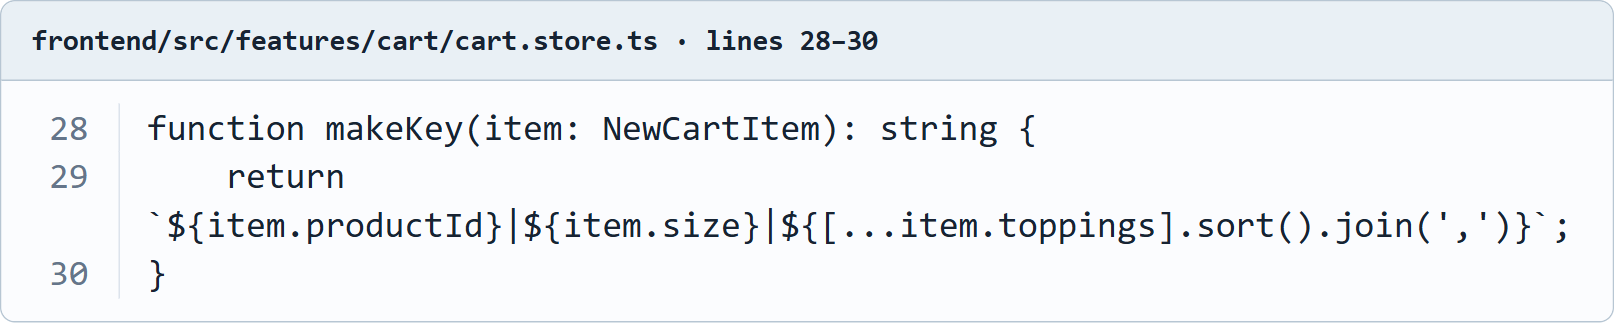
\includegraphics[width=.93\linewidth,height=.24\textheight,keepaspectratio]{assets/catalog-cart/code-key.png}
\caption{Khóa dòng giỏ được chuẩn hóa theo sản phẩm, size và topping}
\vspace{3mm}
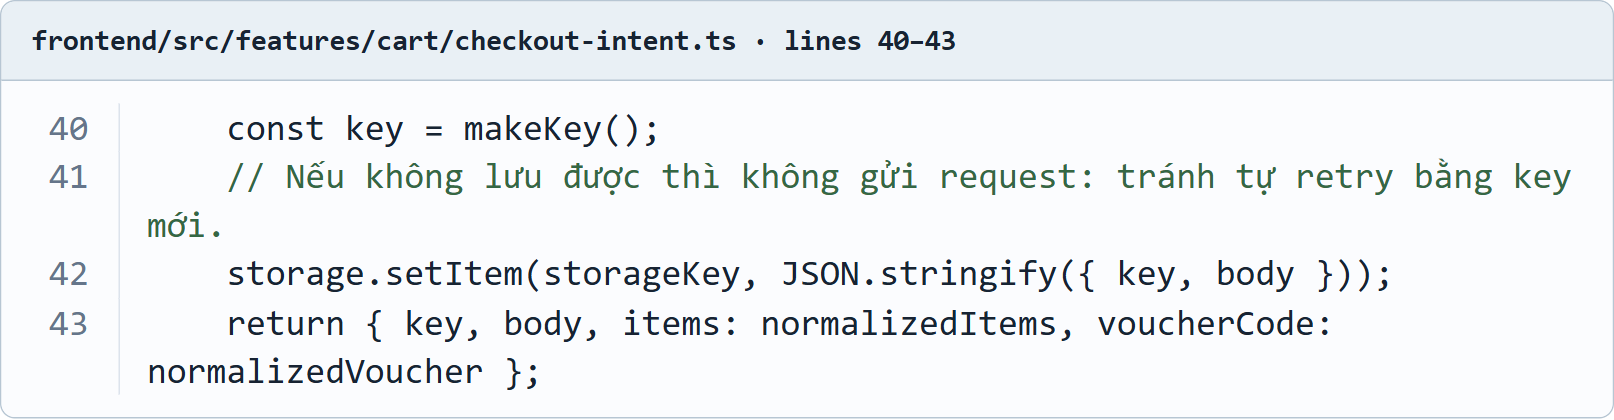
\includegraphics[width=.93\linewidth,height=.24\textheight,keepaspectratio]{assets/catalog-cart/code-intent.png}
\caption{Lưu ý định đặt hàng trước khi gửi để tái sử dụng key khi cần}
\vspace{3mm}
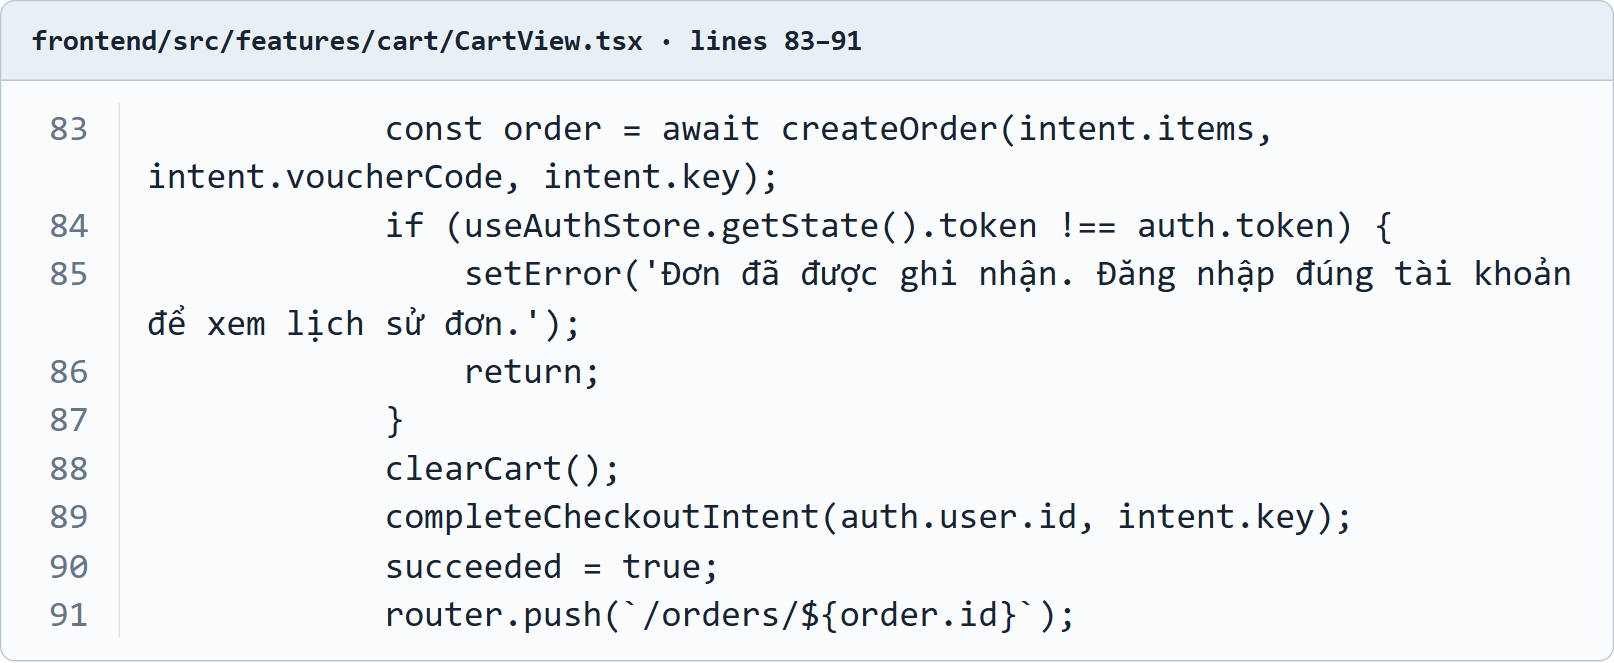
\includegraphics[width=.93\linewidth,height=.25\textheight,keepaspectratio]{assets/catalog-cart/code-submit.png}
\caption{Gửi lựa chọn và chỉ xóa giỏ sau khi backend xác nhận đơn}
\end{figure}
